\subsection{Moment Tensor inversion in SEISAN}
\label{sect:Dreger}
\index{Dreger} 
\index{Moment tensor inversion} 

\textbf{Introduction}

The moment tensor inversion for regional earthquakes implemented in SEISAN uses the well tested Dreger code \citep{dreger2003}.The software has been integrated into SEISAN to take advantage of all the parameters already being part of the SEISAN data base like response, hypocenter and station parameters as well as SEISAN's ability to do instrument correction and filtering. All operations take place through EEV including an optional search for the best hypocentral depth. A tutorial for the original Dreger software including basic information on the principles of the software is found in INF, \texttt{mt\_dreger.pdf}.

\textbf{What data to use}

The program works for regional distances (up to 2000$-$3000 km) where the model can be approximated by flat parallel layers., The inversion will generally work best for events large enough to produce low frequency signals (f$<$0.1 Hz) which means surface or sometimes S-waves (at short distances or for deep events). However theoretically there is no lower magnitude limit since the source time function is a point source. A simple test to see if the data  potentially can  be used at low frequencies, is to apply a filter 0.01 to 0.1 Hz and see if there is a clear signal. A more quantitative test is to make spectral analysis of the S and/or surface waves to observe where the signal to noise ratio approaches 1. There are examples of inversions of small near events (m$=$2$-$3) with frequencies as high as 3 Hz. However, this is not what generally can be expected to work.
It is possible to use any or all of the components Z, R and T, however the T-component is often the most important. It is recommended to use at least 4 stations with at least 6 seismograms, however that is rarely enough to get a reliable solution. Real signals are often more complicated and of longer duration than the synthetic signals, so it is easier to fit  signals with a few simple pulses.

\textbf{Use velocity or displacement}

Our tests show that it does not make much difference for good data. In some cases it might be easier to get stable velocity traces than displacement traces since the effect of the enhancement of  low frequency noise from the conversion to displacement is avoided. Whatever is selected in MULPLT is what is used by all programs. There is a check that there is no discrepancy between the data and the Green's function in terms of displacement and velocity.

\textbf{Technical steps to do MT}

\textbf{Step 1} Select channels to analyze and write out a rotated instrument corrected data file in Helmberger format which is used to make input files to the Dreger program. Note, that all filters used must be 4 pole bandpass Butterworth filters, either one way or two ways. Although MULPLT can generate other filters, they can currently not be used for MT inversion. 

\begin{itemize}
\item Make sure the event is well located and all response files are available. If doubt about depth, fix it in S-filer header line.
\item Start EEV.
\item Plot data filtered, it is easier if filter is fixed.
\item Select channels desired for analysis. Select as many channels as possibly can be used. It is possible later to deselect without going back to MULPLT. NOTE:  You can only make a data set of the channels seen on the screen! See below how to deal with many channels.
\item Rotate channels (if 2 horizontals), check that all channels are rotated (no back azimuths of 999).
\item Select filter band and plot signals instrument corrected and filtered. Start with just filtering the signals e.g. in band 0.01 to 0.1, this gives an idea of which channels have good low frequency signals. A good filter to use is often 0.03 to 0.1 Hz. For small events, a filter of 0.5 to 1.0 might have to be used  Inspect the signals to see if they look reasonable. E.g., the instrument corrected amplitudes should not be very different. At this stage errors in the response files or bad data might be detected. If so correct data and select again. A wrong response can seriously affect the solution.
\item When signals look ok and are displayed instrument corrected, filtered and rotated, press button \texttt{OutW}, and wait for message in to right hand corner 'File \texttt{mulplt.wav finished}'. The Ascii file \texttt{mulplt.wav} has now been written out. It can take some time since it is an Ascii format of real numbers (see below). In a multi-trace window there can be missing data in front of the signals and at the end of the signals for some channels. These gaps are filled out with the DC level.
\item Quit MULPLT. 
\end{itemize}

\textbf{How to deal with many channels}: By default, MULPLT shows 99 channels per screen, but this is often reduced to a smaller number by setting parameter \texttt{NCHAN PER SCREEN} in \texttt{MULPLT.DEF} to a number like 24. So if e.g. 100 channels are available, the data will be shown on several screens. The procedure is then:

\begin{itemize}
\item Select channels to use on each screen. If no channels are selected on a screen, all will be used.
\item When the selection is finished and if there are more channels than fitting on one screen, press N. This will plot all channels on one screen and a file with all channels desired can be made. Pressing N again brings back the original number of channels per screen.
\end{itemize}

At this stage, a file with possible data for analysis has been written out with the original sample rate, instrument corrected (units nm or nm/s) and filtered. The two first letters in the component names has been replaced by RR to indicate reprocessed data. The file can be plotted with MULPLT or from EEV with command pd.

\textbf{Step 2} Create parameters needed for MT

The generation of the Greens function needs a series of parameters including the crustal model, which might be the most critical input. The model used will be taken from the \texttt{STATIONx.HYP} file so it will be possible to use a station file different from the default by either working in a local directory with a local \texttt{STATION0.HYP} or having a \texttt{STATIONx.HYP} in DAT, where x corresponds to the model ID given in the S-file. Note that a \texttt{STATIONx.HYP} file can contain Q and density, but often does not and then default values are used. All parameters will be written in the S-file in the SYNT format (including extra mt-variables), see section on synthetic seismograms and the example below.  The stations selected for analysis will be the stations given in the \texttt{mulplt.wav} file as made under step 1. Default values are given for many parameters. In order to generate parameters, in EEV:

\begin{itemize}
\item 
Give command mtp (p for parameter). All needed parameters are now stored in S-file as well as parameters for the synthetic seismogram programs, since many of these parameters are the same.  An example of the parameters is given below. At this time a backup file of \texttt{mulplt.wav} is made for future reference. The name is \texttt{yyyy-mmdd-hrmm-ss.mulplt.wav}.
\item Edit the S-file to change default parameters to desired values, see example below. Often a first test can be made with the default values. By default, modeling is only done for one depth, but it is possible to test a range of depths by editing the parameter file. It is however recommended to use the default depth from the S-file for the initial test.
\end{itemize}

NOTE: Command \texttt{mtp} does not overwrite any parameters already in S-file. If a completely new set of parameters is needed, all the old ones can be deleted in the S-file or by using command \texttt{mtd}.

\textbf{Step 3} Generate and inspect unfiltered Greens functions.

The Greens functions should now be generated with the parameters given in S-file. In EEV:

\begin{itemize}
\item 
Give command \texttt{mtg} (g for Green's functions). This makes Helmerger format files all.green\$\$\$ with all the time series Greens functions needed for the given data set and the requested depths \$\$\$. By default only one depth is used. This might take some time (minutes) depending on number of points used, however the time is independent of the number of stations used. The default is to generate a 512 point time series which by default is 512 secs long. NOTE: All previous Greens function files are deleted before the new ones are made.
\item Plot the Greens functions with command \texttt{pg} (g for Green). It is useful to check if the Greens functions look "reasonable". NOTE: If Greens functions for several depths have been made, only the Greens function with the largest depth can be plotted in this way (file all.green). The other ones must be plotted directly with MULPLT outside EEV. For component codes, see Dreger documentation in SEISAN. Note that the transverse components TSS and TDS have no P-waves so they appear to start later. Not all models and distances might produce reasonable signals, there should at least there should be some resemblance with the data signals. Note that the signals, starting at the origin time (read from S-file) have been time shifted with the reduction velocity to appear to arrive at similar times. At this stage it might be decided that a different time window or sample rate is needed. Then edit S-file and redo step 3.
\end{itemize}


\textbf{Step 4}  Decide on time window length for analysis.

The Green's functions are typically generated for 512 secs (sample rate 1.0) and typically a smaller window around the signals is used like 200-400 s (default 257 s). From the Greens functions signal, it can be seen how long a minimum window is needed. The window should be longer than the signals. Before inversion, the signals are also time shifted (like the Greens functions are already) with the reduction velocity in order to make the data file smaller.

\begin{itemize}
\item 
Edit S-file and adjust parameter \texttt{MT-NP-USE} to desired length.
\end{itemize}

Note that the all the Green's function files and the time shifted data files do not have accurate absolute time due to time shifting.

\textbf{Step 5}  Make the inversion

The desired time windows from all.green\$\$\$ are filtered by the selected filter and written out. The filtered time shifted window from \texttt{mulplt.wav} are now selected, filtered by a (desired sample rate)/5 Hz antialias filter and resampled to the desired sample rate and written out. The inversion is now performed. All this is done in EEV. NOTE: All data files from previous inversion are deleted before the data selection.

\begin{itemize}
\item 
In EEV, give command \texttt{mti} (i for inversion).
\end{itemize}

The inversion is now done and the results given on the screen. If a range of depths have been selected, inversion will be done for each depth and the inversion will be repeated for the depth with the best fit so this becomes the last inversion, which can be save in S-file. A table of fit parameter (VR) and depth is displayed together with corresponding fault plane solution. If results are good (see later), they can optionally be saved in the S-file. Note particularly the value of Zcor which is how many samples the data has to be shifted to fit with the Greens function.

\textbf{Step 6} Check results

See  Dreger documentation in INF for the explanation of the output. The variance reduction (VR) is shown for each station as well as for all stations. A low value indicates a bad fit and a negative VR might indicate inverted polarity. The most important check is to see how the synthetic seismograms fit the observed seismograms.

\begin{itemize}
\item 
In EEV, give command \texttt{pm}. The plot of overlaid seismograms is now shown. They should be similar. Plot also with fixed scale to see the absolute difference between the traces.
\end{itemize}

The fault plane solution can be plotted (if saved in step 5) with command \texttt{fo}. Compare to any solution from other sources (if given in S-file, see section \ref{sect:pfs} on fps in SEISAN).

\begin{figure}
\htmlimage{scale=2.0}
\centerline{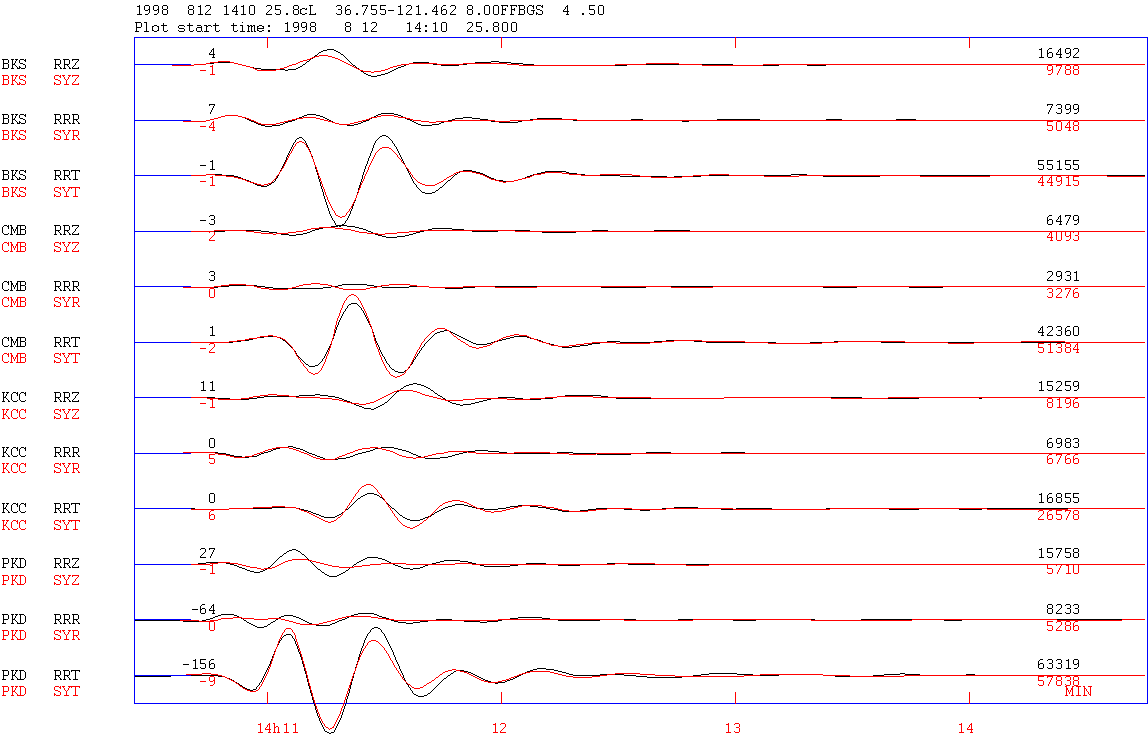
\includegraphics[width=0.9\linewidth]{fig/mt-dreger-1}}
\caption{Plot of original filtered instrument corrected data (blue) compared to the synthetic seismograms (red). The filter used is 0.02 to 0.05 Hz. The plot is made with a fixed scale of 30 000. Note how the T-components dominate the solution. The data is the Dreger test data included in the SEISAN training data. Note that when plotting a file in Helmberger format, the overlay function (see MULPLT section) is turned on automatically for channels starting with SY. }
\label{fig:mt-dreger-1}
\end{figure}

\begin{figure}
\htmlimage{scale=2.0}
\centerline{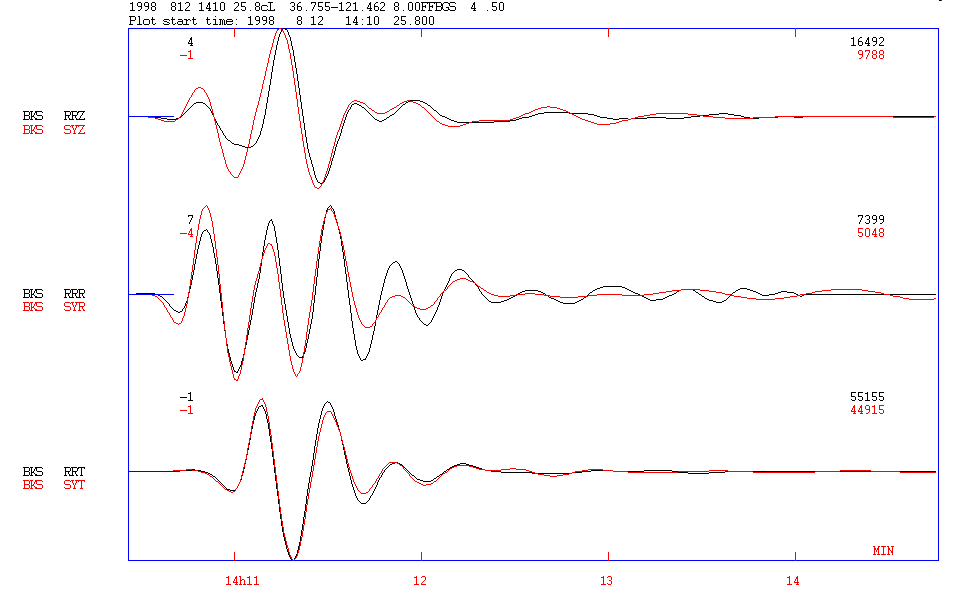
\includegraphics[width=0.9\linewidth]{fig/mt-dreger-2}}
\caption{Same data as shown in previous figure but only for station BKS. The data is now auto scaled. The fit on all channels is quite good. Notice the small amplitude of the radial component.}
\label{fig:mt-dreger-2}
\end{figure}

In the above plots, the original data has been shifted corresponding to the value of Zcor. This means that, for a positive Zcor, the last Zcor data sample on the trace has no data and is replaced by zeros. Similarly if Zcor is negative the first Zcor samples are zero.

\textbf{Judging the results}

See the Dreger documentation for a discussion. Generally the variance reduction VR should be as high as possible.  A bad fit could give an unrealistic moment (and Mw) so that is also an indicator of the quality. 
A good fit is not a guarantee for correct results. If e.g. the gap is large, there might not be sufficiently different data to give a reliable solution, even if the fit is good. The quality given has been assigned by Dreger as follows

\begin{verbatim}
 0 < VR <   20  Quality = 0
20 < VR <   40  Quality = 1
40 < VR <   60  Quality = 2
60 < VR <   80  Quality = 3
80 < VR <  100  Quality = 4
\end{verbatim}

It is necessary to check the solution against the P polarities to confirm that they generally match the solution as wrong alignment can result in inverted solutions. However, it is not to be expected that all the synthetic polarities fit the observed polarities since the fault plane solution from MT (measures overall slip) might be different from fault plane solution with polarities (measures the slip of the initial rupture). Use command fo to plot the solution together with observed polarities recorded in the S-file. 

\textbf{Example of a run of the inversion}



\begin{verbatim}
#    2 12 Aug 1998 14:10 25  L  36.755-121.462 8.00FF  .50     BGS    4  ? mti

***Event to invert***: C:\Seismo\\REA\TEST_\1998\08\12-1410-00L.S199808

Inversion in:             displacement
Number of stations:              4
Number of points to use:       250
Depth:                         8.0
Sample rate:                 1.000
Reduction velocity:            8.0
Filter:                      0.020   0.050

Skip for down sampling for PKD    20
Skip for down sampling for BKS    20
Skip for down sampling for CMB    20
Skip for down sampling for KCC    20

PKD   Distance(km)=   122.0 ShiftVel(s)=     0.1  Offset(sample)=    0
BKS   Distance(km)=   142.0 ShiftVel(s)=     2.5  Offset(sample)=    0
CMB   Distance(km)=   171.0 ShiftVel(s)=     6.2  Offset(sample)=    0
KCC   Distance(km)=   201.0 ShiftVel(s)=     9.9  Offset(sample)=    0

Writing PKD__.green            ShiftVel: Shift in s due to reduction velocity             
Writing BKS__.green            Offset:  Zcor parameter in S-file
Writing CMB__.green
Writing KCC__.green

Output from tdmt_invc:         See Dreger manual for following output

Depth=8
Station Information
Station(0): PKD__.data  R=122.0km  AZI=137.0  W=1.000  Zcor=14
Station(1): BKS__.data  R=142.0km  AZI=331.0  W=1.164  Zcor=13
Station(2): CMB__.data  R=171.0km  AZI=34.0  W=1.402  Zcor=13
Station(3): KCC__.data  R=201.0km  AZI=71.0  W=1.648  Zcor=12
Mo=4.12984e+023
Mw=5.0
Strike=223 ; 130
Rake=18 ; 172
Dip=83; 72
Pdc=98
Pclvd=2
Piso=0
Station(0)=78.607796  4.95437e+010
Station(1)=82.944862  3.37622e+010
Station(2)=82.605667  1.91152e+010
Station(3)=56.903259  6.36377e+009
VAR=7.48972e+006
VR=79.39  (UNWEIGHTED)
VR=79.00  (WEIGHTED)
Var/Pdc=7.668e+004
Quality=3

Update event with new mt solution(n=enter/y) ?
\end{verbatim}

\textbf{How and where parameters are changed for making tests}

After the first parameter file in the S-file has been made, these parameters can only be changed by manually editing the S-file or deleting part or all of the parameters in the S-file and running command \texttt{mtp} again. Possible changes:

\begin{itemize}
\item 
New model: Delete in S-file, edit station file and run \texttt{mtp}. Or correct directly in S-file. However if a new model results in new distances and azimuths, then the station lines should also be  deleted before using \texttt{mtp}. Similarly with the depth line if depth changes.
\item 
New depth: If location is unchanged, only change depth in parameter file and start with step 3.
\item 
Range of depths: Edit S-file depth line.
\item 
New event location: Delete station lines in sfile and start with step 2.
\item 
Take out some stations: Change the ID in the first station line (the one with mt specific parameters), e.g. write xSTATION instead of STATION. Then run inversion again, step 5.
\item 
Take out components for a station: Edit the field \texttt{MT-COMP: TRZ}, see below. Then run inversion again, step 5.
\item 
Change filter: A new data selection in MULPLT must be made with the new filter and the new filter must be written into the S-file. There is a check if filter in S-file corresponds to filter in data file. Then continue with inversion, step 5.
\item 
Add a completely new station: Start from the beginning, this requires complete data selection and computation of Green's functions. The simplest is to delete all parameters with mtd.
\item 
Change from displacement to velocity: Start from the beginning.
\item 
Change sample rate: Change in S-file and start from step 3 making Greens functions. Remember to change the number of points for inversion correspondingly, that is e.g., if sample rate is doubled, number of points must also be doubled to analyze the same length time window.
\item 
Change reduction velocity. Change in S-file and ideally start from step 3. However, starting from step 4 gives the same result provided the time window is long enough, see also below.
\item 
Adjust  time shifts:  Zcor gives the number of samples the data automatically has been shifted to correlate with the Greens function. Check how the synthetic seismograms fit the observed seismograms. This number can be adjusted in the s-file. The number should be Zcor plus or minus a few data points. If zero, the automatic correlation is used. \textit{If real data is seen to the left of the synthetics, reduce Zcor and increase if the data is to the right of the synthetics} (indicated on top of plot as \"Data left. -Zxor\"). Zcor can be positive or negative.
\item 
In general, if deleting a line with parameters, they can be regenerated by command mtp.
\end{itemize}

If a range of depths is used or the new mt solution is updated, the mt is written to 
a file named \texttt{psmeca.in} that can be used to plot the mt solution with 
the GMT program \texttt{psmeca}. With the command\newline
\texttt{psmeca psmeca.in -R10/80/0/42 -JX16/-20 -Sd0.3 -Gred -P -B10f5:"Variance reduction":/1:Depth: $>$ mt.ps}\newline
the double couple part was plottes in figure \ref{fig:mt-depth}. 
Using \texttt{-Sm0.3} will show the mt.

\textbf{Summary of mt related commands in EEV}

\begin{itemize}
\item 
mtp	Make parameters
\item 
mtd	Delete all parameters
\item 
mtg	Make Greens functions
\item 
mti	Make inversion
\item 
pm	Plot observed and synthetics
\item 
pd	Plot mulplt.wav
\item 
pg	Plot greens functions
\item 
fo	Plot fault plane solutions
\end{itemize}

\textbf{Influence of parameters}

\textit{Filters}: Try to find a filter giving a good signal to noise ratio. There can be substantially difference using different filters. 

\textit{Reduction velocity}: It has little influence on the results except that Zcor changes due to relative change in arrival times. It is normally selected to include signals before the P arrival and to include all surface waves. Even different reduction velocity for real and Greens function data does not matter. The use of reduction velocity only has the purpose of reducing the length of the traces by putting events close in time. This is particularly important when using events in with a wide distance range.

\textit{Time window}: The most important is that the time window includes the whole time signal to be inverted. The time window actually used by the program will depend on how close it is to a $2^n$ number. \newline
The correlation is done only with $2^n$ samples. The number of samples selected for correlation can be both larger and smaller than the number of samples in the data file. E.g. if number of samples is between 90 and 181, 128 samples will be used and if between 182 and 362, 256 samples is used etc.\newline
The inversion also seems to use a $2^n$ number and there can, in a few cases, be a radical difference between using e.g. 256 and 257 points in calculating the fit VR, but apparently not the solution itself. The default number of samples to use is therefore 257.   So if the number of samples is near a $2^n$ number, use a number a bit larger than $2^n$. This change in fit is not generally observed, in most cases VR is not affected.\newline
Inspect the Greens function file all.green (command pd) or use MULPLT with all.green\$\$\$ to see how long the Green function signal is and similarly look at the data files. The time shifted data files are STAT.data and can be plotted with MULPLT.

\textit{Sample rate}: Seems to have little influence if well above the frequencies of analyzed data. One or two Hz seems ok for data where the inversion is made for frequencies below 0.1 Hz. For 1 Hz data 4$-$8 Hz or similar (depending on sample rate of original data).

\textit{Number of stations and components}: It is often difficult to get good results with all stations and components. Start with a few stations (even one god one) and gradually add data. Note that changing station configuration also can change the time shift between synthetic seismograms and the data. It is important to have as small a location gap as possible.

\textit{Zcor}: Zcor is calculated by correlating the Greens functions with the data and the synthetic seismograms might need a correction as observed from the overlay seismograms. The Zcor time shift will change with different solutions so there is no final Zcor that will work in all cases. Small changes in Zcor can significantly improve the results. In the worst case, Zcor might have to be large enough to reverse the polarity of a signal or even larger if e.g. P has been correlated with S (small events at higher frequencies). The automatic correlation is what creates most problems. 

\textbf{What can go wrong}

\begin{itemize}
\item 
Very bad fit. This can be caused by the correlation not working well, Signals might be shifted several cycles. Try using a different time window, particularly a longer one.
This can also be cause by a bug which results in a factor 2 wrong sample rate. it is clearly seen whan comparing the synthetics and real data. Just run again usually fixes the problem:
\item 
Crash of inversion program. This might be caused by correlation not working. Zcor for a particular station might have  a value of millions. Do not use the particular station.
\item 
Deselecting components does not always seem to work, then use all 3 component or deselect station.
\item 
The invasion does not start. Use \texttt{Ctrl+c} and start again. 

\end{itemize}

\textbf{Rerunning a previously analyzed event}

The S-filer contains all a parameters used including the start time and duration of the data file so it is possible to extract the same data file for the same channels again. The Green's functions must be regenerated by command mtg. If the user does not delete the backup files (see above) the data file is available as backup file and a question will be given if the previous data file should be used.


\textbf{Running the programs independently of EEV}

Once a first run has been made, the programs can be run independently of EEV using the original parameter files. This can be an advantage if the user wants to change some of the hardwired parameters. However, this can only be done for one depth.

\texttt{FKRPROG\_SEISAN}: The only parameters which might be tested are the group velocities. Dreger is vague about what they should be but their values seem to have some influence on the Greens function. It is also possible to edit other parameters independently like the model.

\begin{itemize}
\item 
Edit the \texttt{green.par\$\$\$} file (\$\$\$ is depth). 
\item 
Run program \texttt{fkrprog\_seisan}: \texttt{fkrprog\_seisan $<$ green.par\$\$\$}
\item 
Convert to time domain by running \texttt{vwint\_seisan}
\end{itemize}

\texttt{TDMT\_INVC\_SEISAN}: The only parameter that cannot be tested through EEV is to make the analysis window smaller than the data window. This sometime improves the results.

\begin{itemize}
\item 
Edit parameter file \texttt{mt\_inv.in}
\item 
Run \texttt{TDMT\_INVC}: \texttt{tdmt\_invc\_seisan}
\end{itemize}

Running in this way, the synthetic file readable by SEISAN is not generated and cannot be updated with the results.

\textbf{Example of parameters in S-file}

\verbatiminput{include/mt.sfile.example}

Most of the parameters are explained under synthetic seismograms. The new ones used only for mt  and other important ones are:\newline
\texttt{DEPTH--}: The first number is start depth, the following number of depth to test and the last number is the increment in depth. The default is one depth only.
\texttt{MT-NP-USE}: Number of points for the inversion, default 257. The number does not have to be $2^n$ but it seems that, in some cases, a number a bit larger than $2^n$ is better than $2^n$ or a bit smaller.\newline
\texttt{NPOINTS}: Number of points in time domain used to make Greens function, default 512. This number must be $2^n$.\newline
\texttt{MTSTART}: Start time of data window used.
\texttt{MT-WINDOW}: Length (s) of data window used.
\texttt{MT-RATE}: Sample rate to use. This rate will be used for Greens function generation and the observed data will be down-sampled to this rate. \textit{NOTE: The rate must have value so only skipping samples in the data can be done}. So the rate 1 can nearly always be used while rate 3 rarely can be used. The time window for the Greens function will then be NPOINTS/MT-RATE. Default 1.0 samples/s.\newline
\texttt{MT-REDVL}: Reduction velocity, default 8 km/s.\newline
\texttt{MT-FILT}: Filters to use for both data and Greens functions. \newline
\texttt{MTOFFSET}: Offset in samples for the data relative to the Greens function. Default 0.\newline
\texttt{MT\_COMP}: Indicate which component to be used. By default all 3 are used, but any combination can be selected. T, R and Z can come in any order but must be within column 76:78.\newline

\textbf{Technical notes}

The Dreger MT inversion essentially consists of a Green's function generation program, \texttt{fkrprog} (in SEISAN called \texttt{fkrprog\_seisan}), several data manipulation programs and scripts using SAC to prepare data for the inversion program \texttt{tdmt\_invc} (in SEISAN called \texttt{tdmt\_invc\_seisan}).  The two key programs have been left nearly unchanged (all changes are clearly marked in programs) while the data manipulation programs mostly have been replaced by standard SEISAN functions (mostly within EEV) and one modified Dreger program \texttt{wvint9} (now called \texttt{wvint\_seisan}) so only 3 programs have been added to SEISAN. A significant change is that Dreger uses cm as a unit while SEISAN uses nm, so software has been changed to nm like elsewhere in SEISAN. 
The Dreger code has no provision for  using less than 3 channels. However, undocumented information indicates that if a data channel has zeros, it is not used and this is how it is implemented in SEISAN. In some cases it does not seem to work well, should be investigated more.
The data and Greens functions in Dregers software are using the Helmberger format, a simple Ascii format without reference to time and channel name. SEISAN will, for simplicity use the same format, but it has been extended to also include channel information, absolute time and an ID of the event being processed (the S-file name), see example below. 

\verbatiminput{include/mt.helmberger}

The two first lines are main headers. The first line has number of channels in file (format i8) and has been extended with, filter band, number of poles and passes and S-file name. Only the number of channels is required information for plotting. The second line gives format of data, extended with help text which in this case is information that file is in displacement (nm). The following two lines are channel headers for each channel. The first channel header has undocumented information. The second channel header has number of samples in channel (i8), sample interval(s)(f10.3), undocumented and starting from column 32, the station code, channel code and start time.

The program flow in SEISAN is

\begin{itemize}
\item 
Plot, rotate, filter and instrument correct signals. This generates an output file \texttt{mulplt.wav}. A parameter is set in MULPLT to enables the output. This file has not been re-sampled.
\item 
Make parameters in S-file (command \texttt{mtp}): Parameters are selected from \texttt{mulplt.wav} (stations to use, filter and whether displacement or velocity), from s-file (depth, distances and azimuths), from station file (model) and some are hardwired. The operation takes place in EEV. At this point the backup data file is made.
\item 
Generate the 10 Greens functions (command \texttt{mtg}): All old Green's functions are deleted and parameter files to \texttt{fkrprog\_seisan} (\texttt{green.par\$\$\$}, \$\$\$ is depth) are made from the S-file (inside EEV), \texttt{fkrprog\_seisan} is run giving an output file with frequency domain Greens functions \texttt{green.out}. This file is converted to a Greens function time domain files, \texttt{all.green}, with \texttt{wvint\_seisan} (modified version of original program \texttt{wvint9}). Since it is assumed there is no explosive component, only 8 of the 10 greens function are written out in time domain (as the original program). \texttt{all.green} is in Helmberger format. Information of using displacement or velocity is read from S-file. 
\item 
Make inversion (command \texttt{mti}). In EEV, same length time windows, one for each station, are extracted from \texttt{all.green} and \texttt{seisan\_mt.out}. Names are \texttt{STA.green} and \texttt{STA.data}. The old \texttt{STA.green} and sta.data are deleted first. The  Greens function files are antialias filtered with a LP filter of 4 poles at (desired sample rate)/5 Hz (not sure it is needed), re-sampled and time shifted, all in EEV. If a channel has been deselected or not available, zeros are written out. The Greens functions are band-pass filtered and anti alias filtered with same filters as used for the data. The parameter file (\texttt{mt\_inv.in}) for the inversion program \texttt{tdmt\_invc\_seisan} is made (in EEV) and the inversion program started from EEV. The inversion program makes an output file with signals and synthetics (\texttt{synt.out}) which is converted to Helmberger format file \texttt{synt\_seis.out} in EEV. Command \texttt{pm} will plot this directly in EEV. File \texttt{mt\_inv\_redi.out}  (as the original) has details of the results and  is read by EEV to optionally get results back into the S-file.
\end{itemize}

\textit{Fkrprog\_seisan}: The parameter file format has been changed to include station names and the s-file name.\newline
\textit{Tdmt\_invc\_seisan}: The program has minor changes to accept new Helmberger format (it also reads the original format). It did not work properly under Windows with more then 450 points, so memory allocation was doubled to fix this. The plotting routine has been simplified to only write original and synthetic seismograms.

To get correct overlay, the channels must be sorted alphabetically. MULPLT turns on sorting (normally set in MULPLT.DEF) if the filename is synt\_seis.out.
\index{synt\_seis.out} \index{Sorting in MULPLT}

The SEISAN implementation is dimensioned to max 99 stations.

\begin{figure}
\htmlimage{scale=2.0}
\centerline{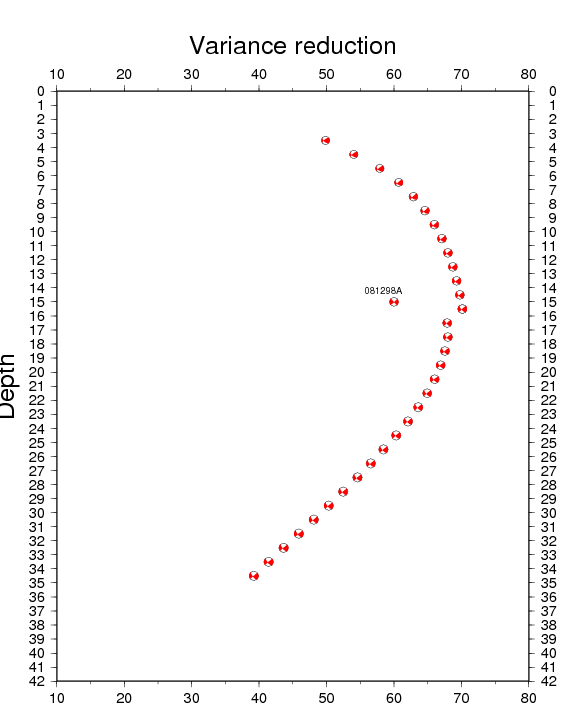
\includegraphics[width=0.9\linewidth]{fig/mt-depth}}
\caption{The double couple part of the moment tensor solution shown with respect to the 
variance reduction at different depths. The GCMT solution is also shown with 
arbitrary variance reduction. This figure was made with the GMT program psmeca, se text.}
\label{fig:mt-depth}
\end{figure}


